\chapter{КОНСТРУКТОРСКАЯ ЧАСТЬ}
\label{cha:ch_1}

\section{Формирование облика комплекса}
Облик современного противотанкового ударного комлпекса на базе БПЛА формируется двумя блоками факторов - обликом современных БПЛА, несущих ПТУР, и обликом современных целей ПТУР. В данной работе в качестве целей ПТУР рассматриваются современные танки, так как они несут наиболее совершенные средства защиты от поражения.

\subsection{Облик современных \\ударно-разведывательных БПЛА}
В настоящее время многие развитые  и некоторые развивающиеся страны мира имеют в распоряжении ударно-разведывательные БПЛА. Этот класс беспилотных летательных аппаратов можно приблизительно характеризовать по следующим признакам:

\begin{enumerate}[1.]
	\item Дозвуковая скорость полета;
	\item Максимальное полетное время более 10 часов;
	\item Потолок высоты более 5 км;
	\item Боекомплект, состоящий из высокоточного оружия.
\end{enumerate}

Боевыми задачами БПЛА данного класса являются:
\begin{enumerate}[1.]
	\itemОбнаружение объектов, бронетехники и личного состава противника;
	\itemЦелеуказание и корректировка огня артиллерии и РСЗО;
	\itemПодсветка целей для ракетных ударов;
	\itemСамостоятельное уничтожение бронетехники и слабозащищенных объектов противника.
\end{enumerate}

В силу невысокой защищенности от огня противника и низкой скорости, данный тип беспилотных летательных аппаратов слабо защищен от современных средств ПВО противника, таким образом, их использование возможно только при уничтожении или подавлении ПВО противника или же при отсутствии у того современных комплексов ПВО.

Своеобразным законодателем мод в области разведывательно-ударных БПЛА являются Соединенные Штаты Америки. В 1994 году совершил свой первый полет MQ-1 Predator (рисунок \ref{fig:predator1}). В самом начале БПЛА разрабатывался как исключительно разведывательный, однако в 2001 году военные осуществили проект по установке ракет Hellfire на MQ-1, и до сих пор данная модель БПЛА используется в американской армии. На данный момент компания-разработчик комплекса General Atomics выпустила две новые модели в данной ветке: MQ-9 Reaper (Predator B) и General Atomics Avenger (Predator C), изображенные на рисунках \ref{fig:reaper1} и \ref{fig:avenger1} соответственно. Отличие моделей заключается в количестве внешних подвесов, грузоподъемности и практическом потолке применения БПЛА.

\begin{figure}[h]
\begin{center}
	\begin{minipage}[h]{0.4\linewidth}
		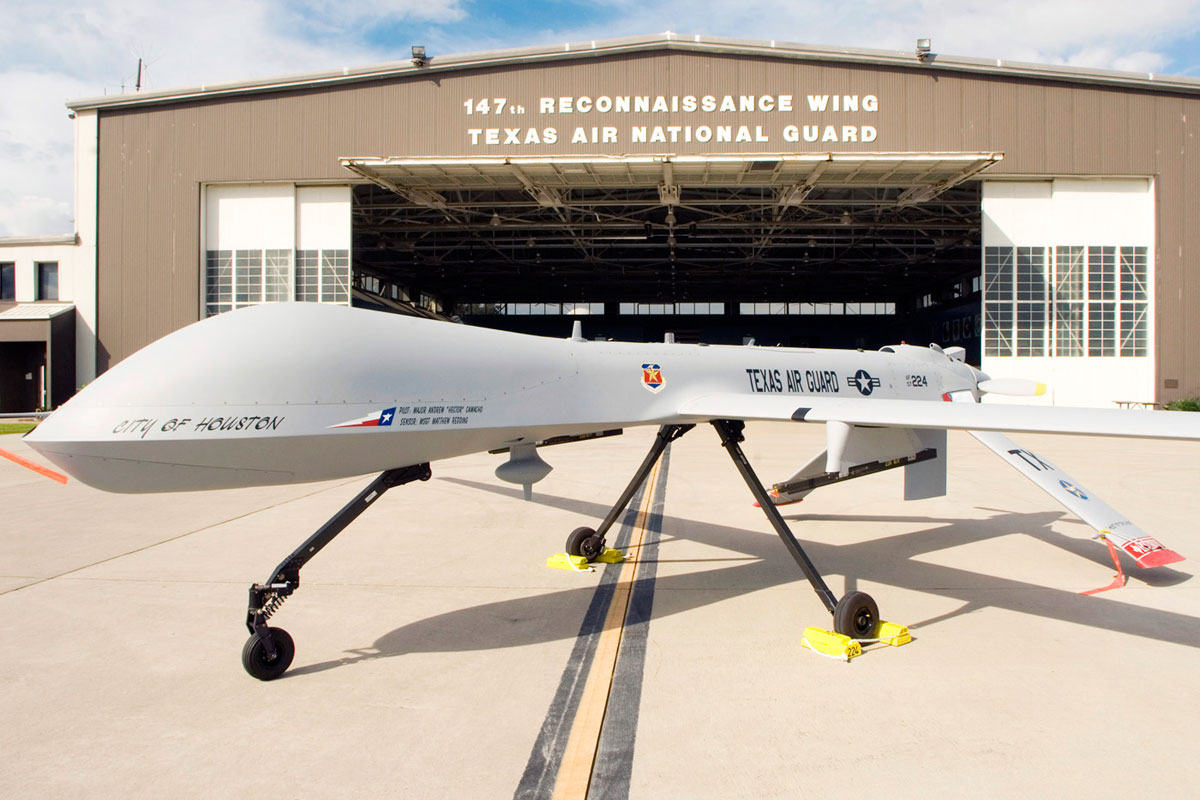
\includegraphics[width=1\linewidth]{predator.jpg}
		\caption{Внешний вид MQ-1 Predateor}
		\label{fig:predator1}
	\end{minipage}
	\begin{minipage}[h]{0.4\linewidth}
		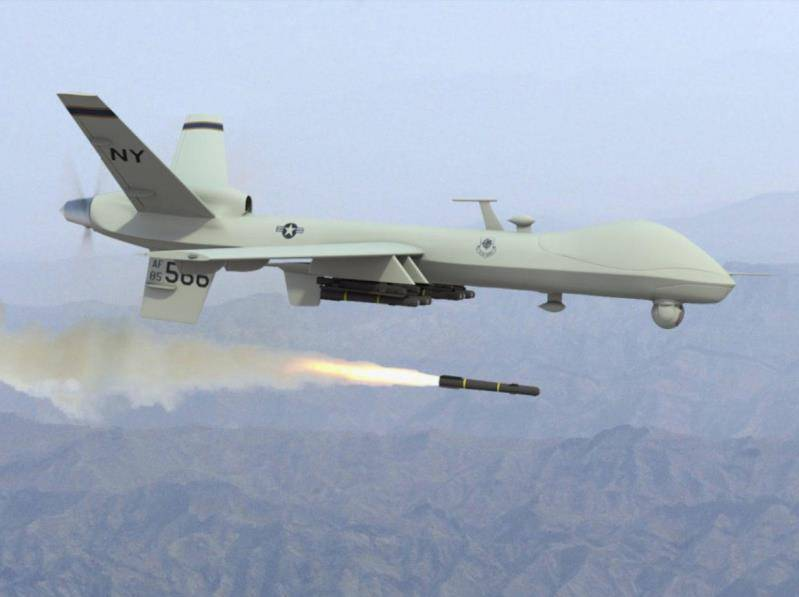
\includegraphics[width=1\linewidth]{reaper.jpg}
		\caption{Внешний вид MQ-9 Reaper}
		\label{fig:reaper1}
	\end{minipage}
\end{center}
\end{figure}

Остальные страны в той или иной степени повторяют опыт США – либо армии стран-партнеров напрямую закупают американские ударно-разведывательные беспилотные летательные аппараты, либо занимаются созданием близких по характеристикам БПЛА. К последним можно отнести китайский «Wing Loong» и российский «Дозор-600».

Особенностью вооружения данного класса БПЛА является то, что вооружение находится в основном на внешних подвесах, число которых сильно ограничено (у первых MQ-1 их было всего два – по штуке на крыло). Также важны весовые характеристики из-за ограниченной грузоподъемности БПЛА. Габаритами ПТУР определяется возможность закрепить на одном подвесе несколько ракет сразу.
\begin{figure}[h]
	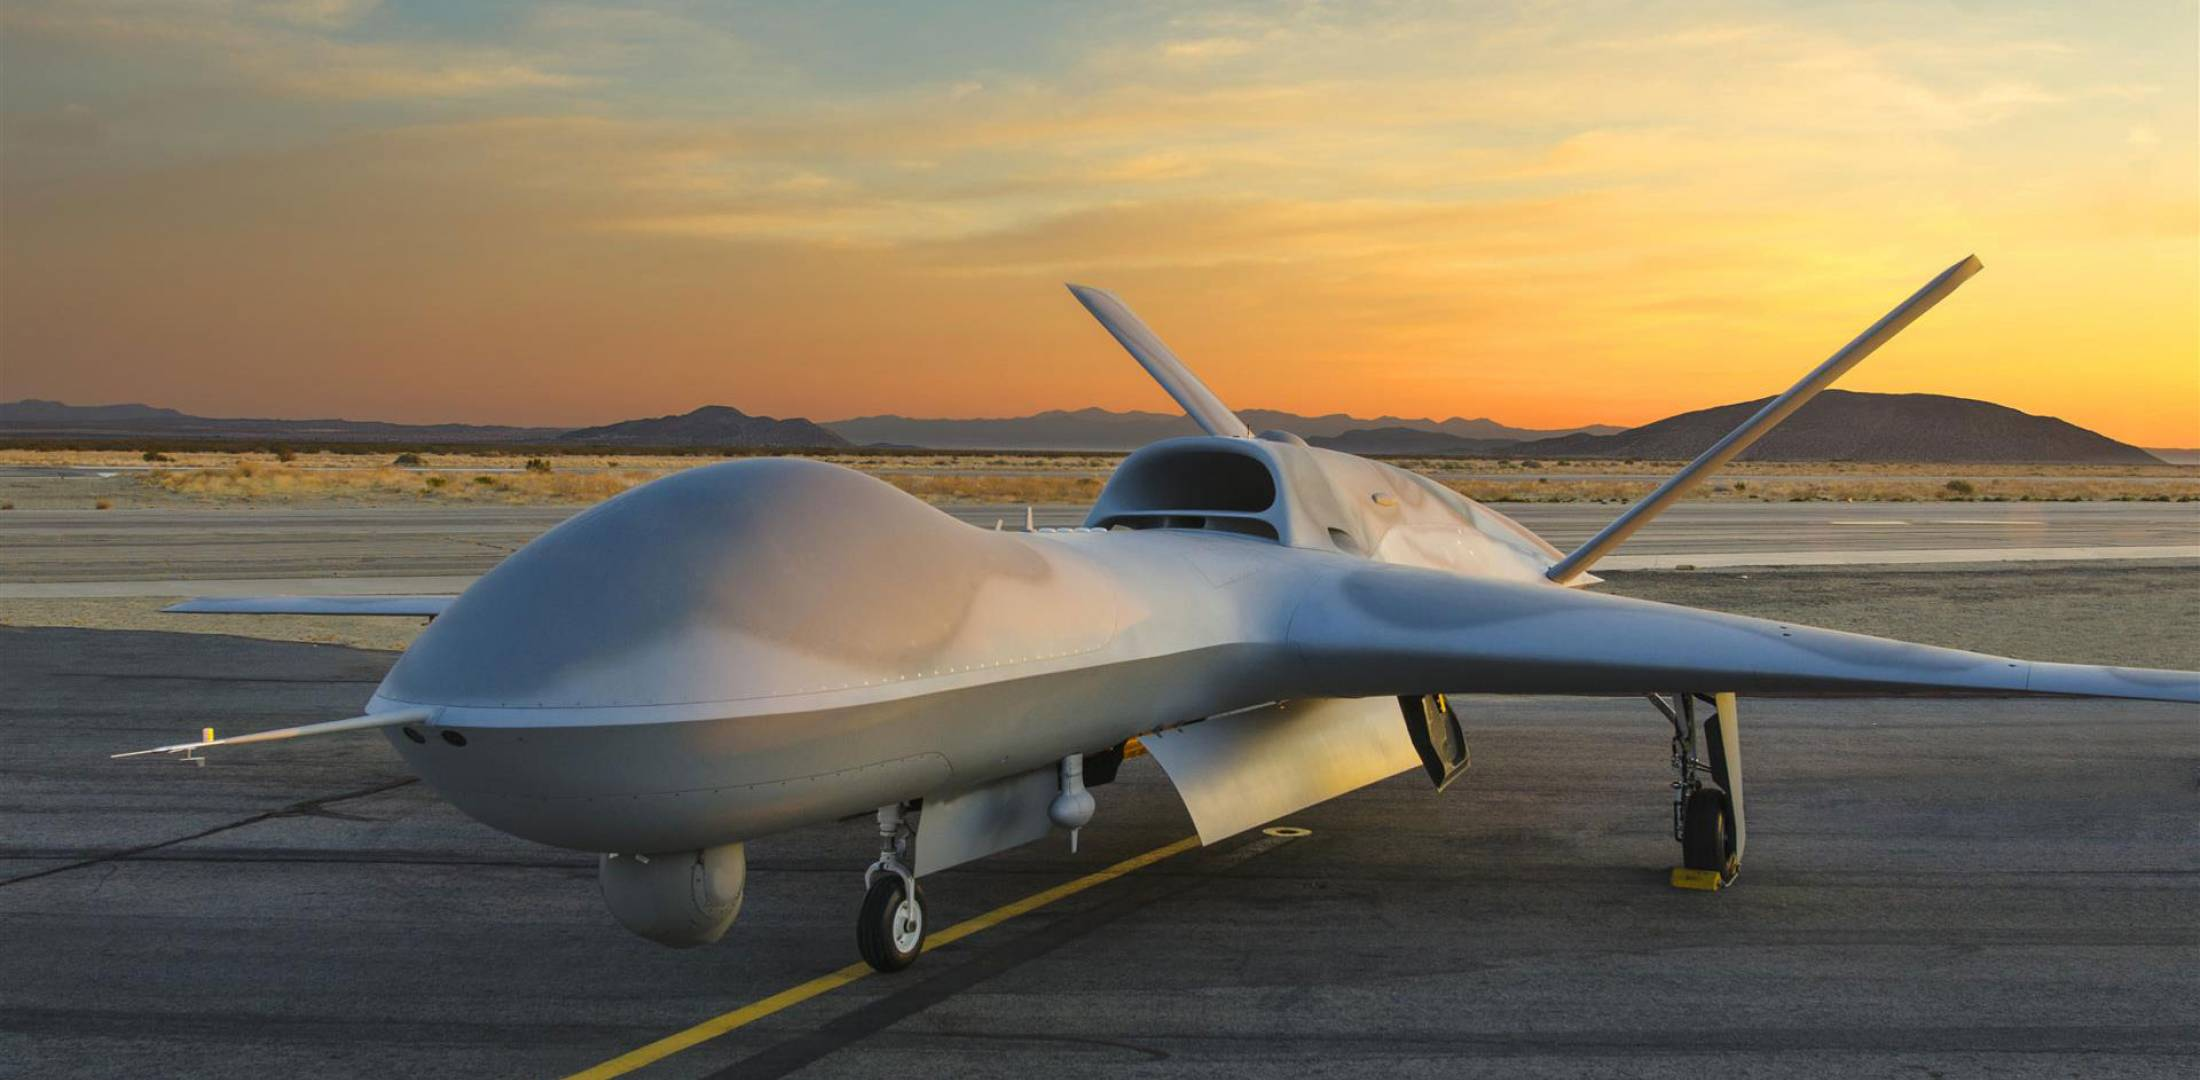
\includegraphics[width=\linewidth]{avenger.jpg}
	\caption{Внешний вид General Atomics Avenger}
	\label{fig:avenger1}
\end{figure}

Американский опыт демонстрирует следующее: сначала на MQ-1 устанавливали тяжелые и мощные ракеты AGM-114 Hellfire с лазерным наведением, однако военных не устроил малый боекомплект БПЛА и дороговизна каждой ракеты по сравнению с их типичными целями, а также количество сопутствующего ущерба, производимого каждым пуском мощного ПТУР (разрушение дорог и построек). Поэтому в скором времени после начала боевого применения кампания Raytheon разработала ПТУР AGM-176 Griffin меньшего калибра и массы. Теперь вместо двух ПТУР Hellfire БПЛА MQ-1 мог взять с собой шесть ПТУР Griffin, а ущерб от одного пуска не был столь разрушительным. Также AGM-176 имеет возможность наведения на цель по GPS и ИНС, что позволяет точно поражать неподвижные объекты без необходимости подсветки цели БПЛА.

\clearpage
\subsubsection{Влияние облика БПЛА \\на ТТХ используемых ПТУР}
Описанные выше особенности носителей ПТУР приводят к следующим требованиям:
\begin{enumerate}[1.]
	\item Необходимость наведения на цель, в том числе подвижную, по отраженному лазерному лучу;
	\item Максимальная дальность полета более 5 км при пуске с минимальной высоты;
	\item Возможность применения в тёмное время суток;
	\item Низкая заметность ПТУР во всех диапазонах для обеспечения как можно большей защищенности БПЛА от ПВО;
	\item Возможность наведения на цель при помощи GPS и/или ИНС;
	\item Малая масса и габариты, позволяющие БПЛА перевозить более 1 ПТУР на одном подвесе.
\end{enumerate}

\clearpage
\subsection{Облик современных танков}
Танки – самые защищенные из бронированных целей ракет БПЛА, поэтому тактико-технические характеристики этих ПТУР определяются, в основном, защищенностью современных и перспективных основных боевых танков.
Средства защиты танков сегодня можно разделить на 4 категории:
\begin{enumerate}[1.]
	\item Бронирование танка;
	\item Динамическая защита;
	\item Комплексы активной защиты (КАЗ):
	\begin{enumerate} [3.1.]
		\item Комплексы оптико-электронного противодействия (КОЭП);
		\item Системы с отстреливаемыми защитными зарядами.
	\end{enumerate}
\end{enumerate}

\subsubsection{Бронирование танка}
Броня – самый старый и естественный способ защиты экипажа и узлов боевой машины от поражения противником. В настоящее время стандартом танковой брони является комбинированная многослойная броня, состоящая из двух или более слоев металлических и неметаллических материалов. Такая броня разработана для защиты от кумулятивных боеприпасов и бронебойных оперенных противотанковых снарядов (БОПС).

Вне зависимости от действительного материала брони, показателем защищенности танка является так называемая эквивалентная толщина брони. Эквивалентная толщина – толщина листа гомогенной стали в миллиметрах, обеспечивающего такую же защищенность танка. Эту величину удобно использовать в расчетах эффективности различного вооружения против танка, а также при формировании ТТЗ на новые образцы вооружения.

На рисунке \ref{fig:leo2_armor} представлено бронирование современного танка ФРГ Леопард-2 в модификациях A0-A4. Данные модификации от последующих (в настоящий момент последней является A7V2) отличает полное отсутствие динамической защиты танка.

\begin{figure}[h]
	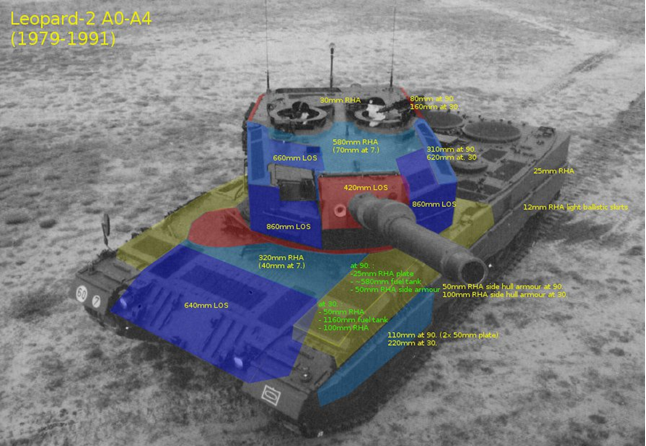
\includegraphics[width=\linewidth]{leo2_armor}
	\caption{Бронирование ОБТ Leopard-2 A0-A4}
	\label{fig:leo2_armor}
\end{figure}

Можно отметить крайне серьезное бронирование передней части крыши башни, однако задняя её часть бронирована слабее из-за наличия на ней приборов танка и люков экипажа.

Тенденция максимального бронирования передней части башни и корпуса и более слабого бронирования верхней проекции танка имела место всю историю танкостроения, и имеет место сейчас.

\subsubsection{Динамическая защита}
Динамическая защита (ДЗ)– более современный способ повышения защищенности танка. Суть ДЗ заключается в размещении поверх основной брони металлических контейнеров, содержащих элементы динамической защиты. Сегодня существует несколько разновидностей динамической защиты, большую их объединяет наличие в элементах ДЗ взрывчатого вещества, которое подрывается при разрушении контейнера и препятствует поражению носителя, снижая кинетическую энергию поражающего боеприпаса или разрушая кумулятивную струю. Такие системы, в основном, применяются на постсоветских танках.

Также существуют системы ДЗ, не содержащие в себе взрывчатого вещества. В этом случае снижение энергии поражающего боеприпаса достигается за счет механической энергии деформированных металлических пластин, содержащихся в ЭДЗ. Таким образом, достигается такой же эффект, как и в случае использования ДЗ со взрывчатым веществом.

На рисунках представлено размещение различных ЭДЗ на современных основных боевых танках.
Как можно заметить, в классических ОБТ с помощью динамической защиты так или иначе повышают защищенность бортов и лобовой части корпуса и башни. Отсутствие ДЗ, к примеру, на корме танка M1A2 Abrams (рисунок \ref{fig:abrams_armor}) с комплектом TUSK объясняется возможными негативными последствиями, которые оказывает срабатывание ДЗ на двигательную установку танка.
\begin{figure}[h]
	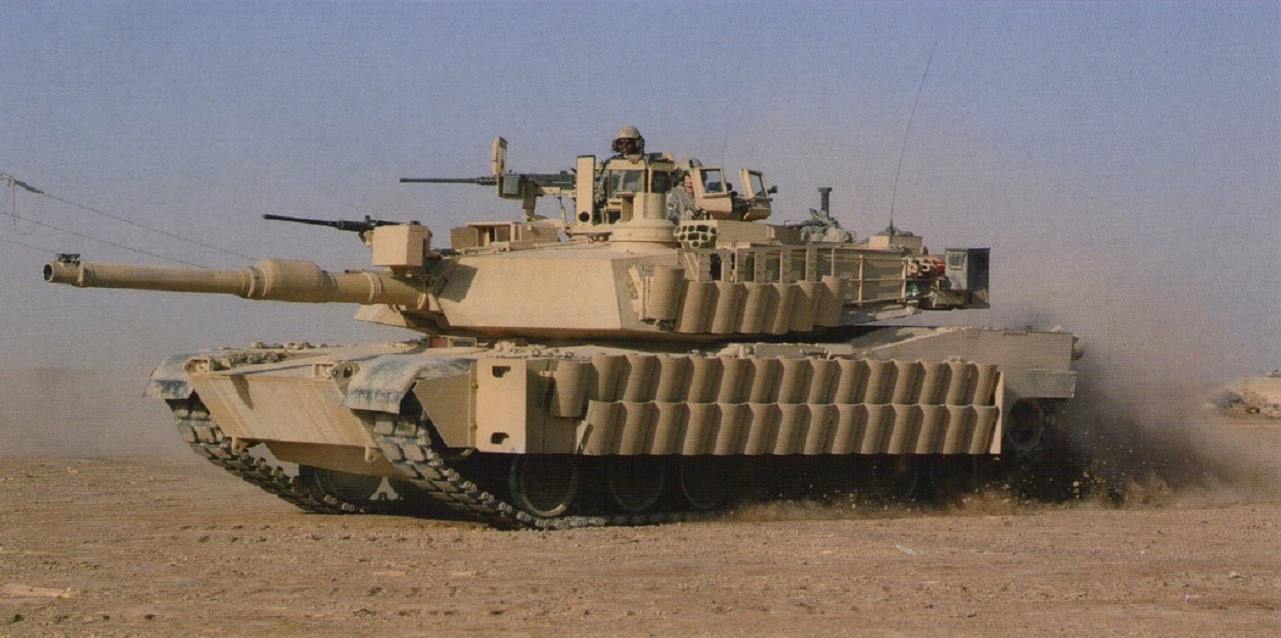
\includegraphics[width=\linewidth]{abrams_armor}
	\caption{Размещение элементов ДЗ на M1A2 Abrams\\с комплектом TUSK (США)}
	\label{fig:abrams_armor}
\end{figure}

По этим же причинам ограничено использование ДЗ на крыше танка, так как бронирование там слабее, чем на корпусе. Также на крыше располагается вспомогательное вооружение танка (зенитные пулеметы) и различные электронные средства, а также люки экипажа. Эту тенденцию можно наблюдать на классических танках Т-72 и Т-84У, схемы размещения элементов ДЗ на которых представлены на рисунках \ref{fig:t72_armor} и \ref{fig:oplot_armor} соответственно.

Таким образом, большинство современных ОБТ имеет слабость в защищенности верхней проекции как собственно броней, так и средствами динамической защиты.

Исключением из этого ряда является перспективный российский танк Т-14 «Армата»: так как башня у него необитаемая, вся её верхняя поверхность покрыта блоками ДЗ, которые можно увидеть на рисунке \ref{fig:armata_armor}.

\begin{figure}[h]
\begin{center}
	\begin{minipage}[h]{0.4\linewidth}
		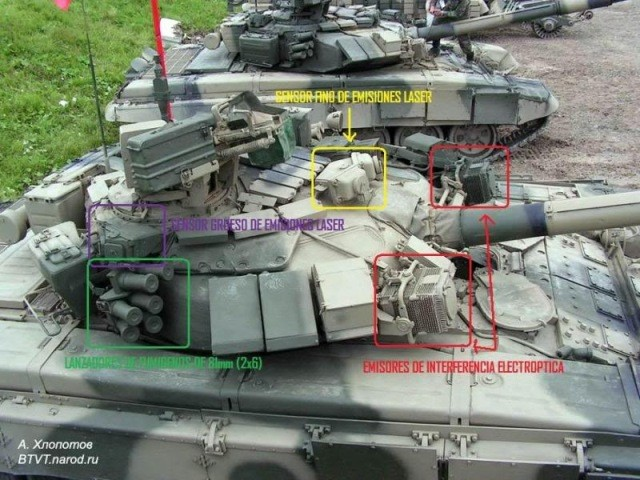
\includegraphics[width=1\linewidth]{t72_armor}
		\caption{Размещение элементов ДЗ на Т-72}
		\label{fig:t72_armor}
	\end{minipage}
	\begin{minipage}[h]{0.4\linewidth}
		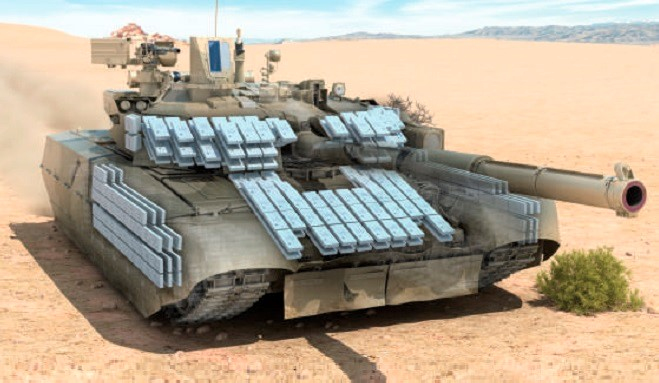
\includegraphics[width=1\linewidth]{oplot_armor}
		\caption{Размещение элементов ДЗ на Т-84У "Оплот" (Украина)}
		\label{fig:oplot_armor}
	\end{minipage}
\end{center}
\end{figure}

\begin{figure}[h]
\begin{center}
	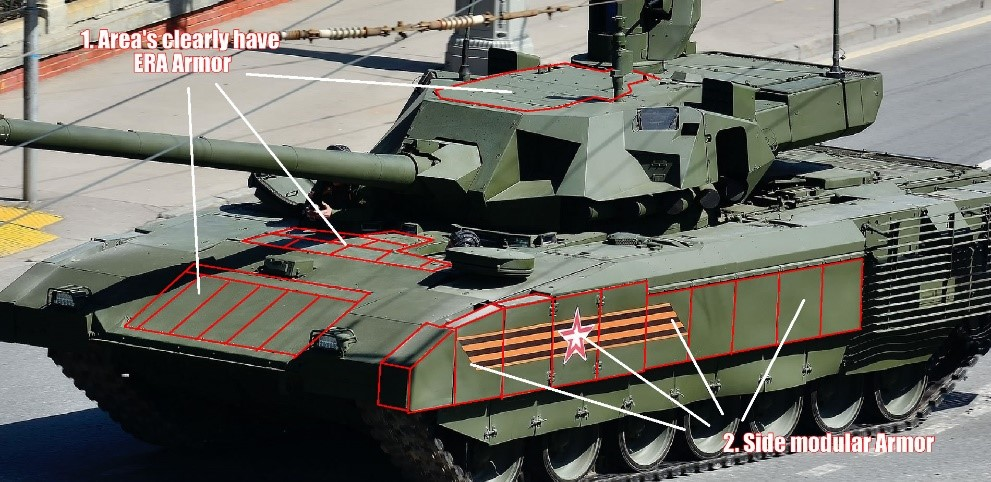
\includegraphics[width=\linewidth]{armata_armor}
	\caption{Размещение элементов ДЗ на Т-14 "Армата"}
	\label{fig:armata_armor}
\end{center}
\end{figure}
\subsubsection{Комплексы активной защиты}
Комплексы активной защиты (КАЗ) – системы, позволяющие обнаружить приближающийся противотанковый боеприпас и поставить помехи, уничтожающие цель или, по меньшей мере, сильно ослабить действие атакующего боеприпаса.

Как разновидность КАЗ, существуют системы оптико-электронного подавления, к ним относится российская «Штора-1». Данные системы позволяют подавлять координаторы наведения устаревших ПТУР – координаторы получают ложные сигналы от комплекса, и ракета врезается в землю или пролетает мимо. Такие системы эффективно работают против устаревших комплексов (Milan, HOT, «Малютка», «Конкурс» и т.д.), однако против новых систем они неэффективны. Поэтому на перспективные российские танки (Т-90СМ) данные системы уже не устанавливаются

Наибольшую опасность для противотанковых снарядов составляют КАЗ с отстреливаемыми элементами, к ним относятся комплексы «Дрозд», «Арена», Quick Kill, Trophy и т.д.
Большинство комплексов активной защиты защищает танк по кругу или части круга, оставляя для противотанковых боеприпасов возможность поразить танк сверху. Исключением из КАЗ, по некоторым данным, является израильский Trophy, создающий сплошную сферу вокруг танка, в которой подлетающие боеприпасы могут быть обнаружены и уничтожены. Однако вызывает вопросы низкий радиус действия Trophy – отстреливаемые элементы отстреливаются при подлете боеприпаса на расстояние порядка 2 м от танка, что, в случае использования, например, AGM-114 Hellfire с осколочно-фугасной БЧ, может означать повреждение внешних систем танка, включая сам комплекс Trophy.

\clearpage
\subsubsection{Влияние облика современных танков\\на ТТХ ПТУР}
Оптимальным способом поражения современных основных боевых танков является поражение их в верхнюю проекцию, так как
\begin{enumerate}[1.]
	\item Бронирование верхней проекции традиционно слабее лобового и бортового;
	\item Установка ДЗ на крышу затруднена и производится редко;
	\item Многие комплексы активной защиты не способны работать против боеприпасов, поражающих танк сверху.
\end{enumerate}

В случае использования в качестве носителя ПТУР ударно-разведывательного беспилотного летательного аппарата, задача поражения бронетехники сверху упрощается в связи с положением носителя при стрельбе.
Таким образом, особенности целей ПТУР приводят к следующим требованиям:
\begin{enumerate}[1.]
	\item Необходимость реализации манёвра для поражения целей в верхнюю проекцию;
	\item Бронепробитие на уровне 800 мм по нормали.
\end{enumerate}

\clearpage
\subsection{Обзор существующих образцов ПТУР,\\применяемых на БПЛА}
Так как основным разведывательно-ударным БПЛА, несущим на себе противотанковое вооружение, является Predator и его копии и модификации, основным противотанковым средством таких БПЛА является классический ПТУР AGM-114 Hellfire и более современный ПТУР AGM-176 Griffin.

Страны, напрямую не эксплуатирующие американские ударно-разведывательные БПЛА, вооружают свои образцы похожими по своим характеристикам противотанковыми управляемыми ракетами. В частности, Китайский ударно-разведывательный беспилотный летательный аппарат Wing Loong вооружен идентичным Hellfire по массе, калибру и системе наведения ПТУРом AFT10 (HJ-10), который ранее устанавливался на боевые вертолеты.
\subsubsection{AGM-114 Hellfire}
Данный образец выбран в качестве вооружения ударно-разведывательных беспилотных летательных аппаратов, так как им же вооружаются ударные вертолеты США.
ПТУР представлен в разрезе на рисунке \ref{fig:hellfire1}.
\begin{figure}[!h]
\begin{center}
	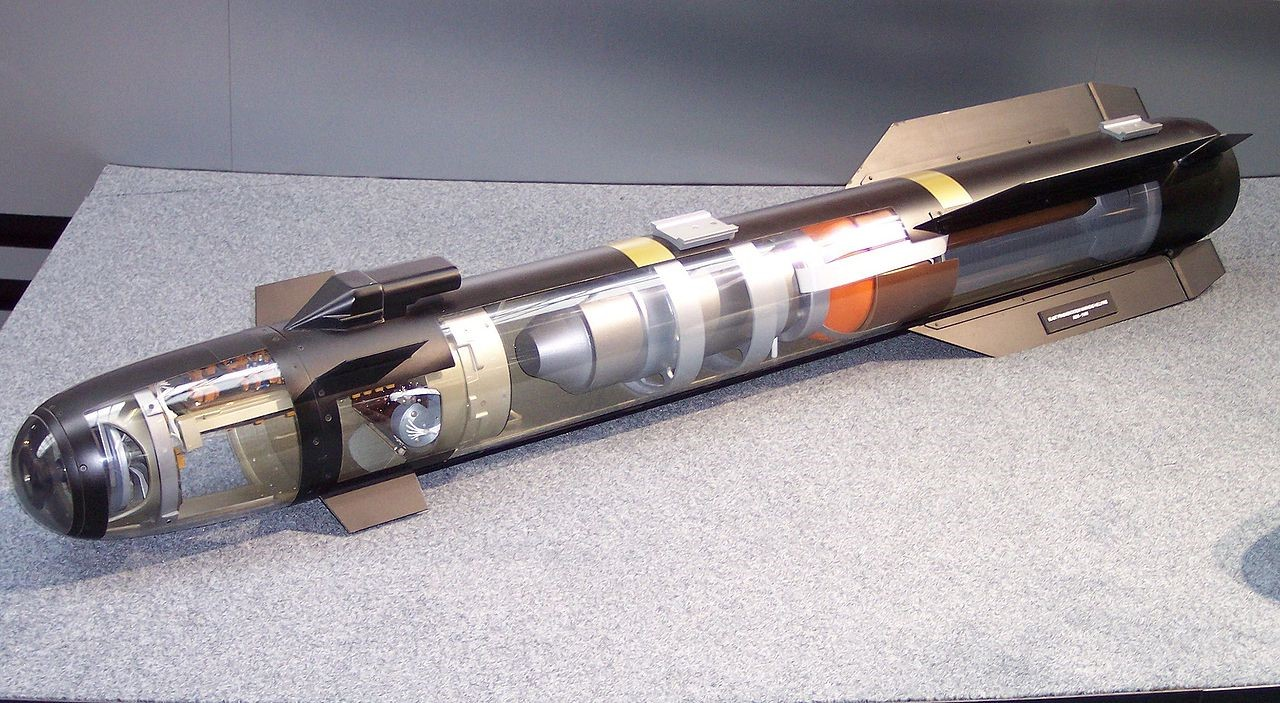
\includegraphics[height=7cm]{hellfire1}
	\caption{AGM-114 Hellfire}
	\label{fig:hellfire1}
\end{center}
\end{figure}
ТТХ образца представлены в таблице \ref{tab:hellfire_stats}
\begin{table}[!h]
	\begin{center}
		\caption{ТТХ ПТУР AGM-114 Hellfire}
		\begin{tabular}{|l|l|}
  		\hline
		Калибр, мм & 178 \\ \hline
		Стартовая масса, кг	& 50 \\ \hline
		Тип БЧ	& Кумулятивная \\ \hline
		Система наведения & Полуактивная лазерная ГСН \\ \hline
		Масса БЧ, кг & 9 \\ \hline
		Максимальная дальность, км & 20 \\ \hline
		Максимальная скорость, м/с & 440 \\ \hline
		Год принятия на вооружение & 1984 \\ \hline
		\end{tabular}
		\label{tab:hellfire_stats}
	\end{center}
\end{table}

\subsubsection{AGM-176 Griffin}
Данный образец изначально разрабатывался как недорогая система, использующая в себе наработки предыдущих образцов: FGM-148 Javelin и AIM-9X Sidewinder. За счет уменьшения калибра по сравнению с Hellfire, разработчики добились уменьшения сопутствующего ущерба при применении ПТУР, а также обеспечили возможность крепления трех ПТУР на одном внешнем подвесе MQ-1 Reaper.

Также данный ПТУР, в отличие от предшественника, можно наводить на неподвижные цели с помощью ИНС и GPS.

Внешний вид ПТУР представлен на рисунке \ref{fig:griffin1}
\begin{figure}[!h]
	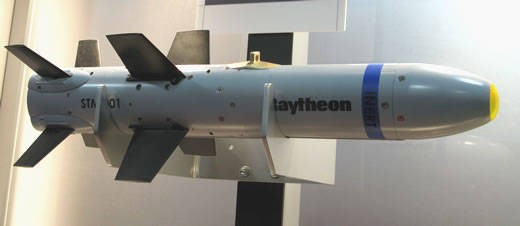
\includegraphics[width=\linewidth]{griffin}
	\caption{AGM-176 Griffin}
	\label{fig:griffin1}
\end{figure}

ТТХ образца представлены в таблице \ref{tab:griffin_stats}
\begin{table}[!h]
	\begin{center}
		\caption{ТТХ ПТУР AGM-176 Griffin}
		\begin{tabular}{|l|l|}
  		\hline
		Калибр, мм & 140 \\ \hline
		Стартовая масса, кг & 20 \\ \hline
		Тип БЧ & Кумулятивная \\ \hline
		Система наведения & Полуактивная лазерная ГСН, GPS, ИНС \\ \hline
		Масса БЧ, кг & 5.9 \\ \hline
		Максимальная дальность, км & 18 \\ \hline
		Максимальная скорость, м/с & дозвуковая \\ \hline
		Год принятия на вооружение & 2008 \\ \hline
		\end{tabular}
		\label{tab:griffin_stats}
	\end{center}
\end{table}
\subsection{Вывод}
В настоящее время разведывательно-ударные БПЛА являются серьезным средством борьбы с танками противника из-за своей относительной дешевизны и отсутствии риска для оператора. Современные ПТУР, которые устанавливаются на такие беспилотные летательные аппараты, могут иметь меньшую массу и габариты по сравнению с ПТРК, запускаемыми с поверхности земли из-за более слабой защищенности их целей в верхней проекции. Также уменьшение калибра позволяет снизить стоимость ракеты, увеличить объем вооружения БПЛА и снизить сопутствующий ущерб при применении комплекса в целом.

Выработанные требования к ТТХ проектируемого ПТУР:
\begin{enumerate}[1.]
	\item Реализация маневра для поражения целей в верхнюю проекцию
	\item Возможность наведения на цель, в том числе подвижную, с помощью полуактивной лазерной ГСН по отраженному лучу или активной ГСН
	\item Бронепробитие на уровне 800 мм по нормали
	\item Максимальная дальность полета более 4 км с минимальной высоты пуска
	\item Низкая заметность во всех диапазонах
	\item Возможность применения в темное время суток
\end{enumerate}

\clearpage
\section{Устройство комплекса}
В состав авиационного комплекса вооружения входят:
\begin{enumerate}[1.]
	\item БПЛА – носитель.
	\item Дозвуковая противотанковая управляемая ракета.
\end{enumerate}

Ракета состоит из трёх отсеков. Первый отсек – полуактивная лазерная головка самонаведения, закрытая прозрачным обтекателем. Во втором отсеке находится кумулятивная боевая часть, взрыватель, ботовая система управления и батареи питания. Четвертый отсек – твердотопливная двигательная установка.

Конструкция ракеты модульная, поэтому каждый отсек может быть заменен независимо от всего изделия. Отсеки друг с другом соединяются винтами.
\subsection{Устройство отсеков ПТУР}
\emph{Отсек 1. Инфракраснaя лазерная головка самонаведения.}

Головка самонаведения имеет обтекатель оживальной формы, прозрачный для ИК-лучей, и состоит из координатора и электронного блока. Головка самонаведения соединена с блоком управления проводами, уложенными в гаргрот.

\emph{Отсек 2. Боевая часть и система управления.}

Система управления и батарея созданы в виде одного блока и устанавливаются в отсек в первую очередь. Далее, после монтирования индукционных рулевых машинок и взрывателя, в ПТУР вкладывается кумулятивная боевая часть. После монтажа боевой части, к ПТУР прикручивается головка самонаведения, предварительно соединенная кабелями блоком управления. Также в блоке управления есть разъем для кабеля, по которому поступает сигнал от носителя.

\emph{Отсек 3. Двигательная установка.}

Двигатель – твердотопливный одноступенчатый. После отделения ракеты от носителя он обеспечивает её разгон до маршевой скорости. Далее ракета управляется с помощью аэродинамических рулей и поражает цель с выключенным двигателем.

\emph{Планер.}

Рули и крылья ПТУР расположены в одних плоскостях; по аэродинамической схеме «утка». Корпус ПТУР выполнен из лёгкого дюралевого сплава, способного выдержать нагрузки при полёте.

\subsection{Описание работы комплекса}
Пуск и управляемый полет ПТУР осуществляются следующим образом. После обнаружения системой поиска (дальность 10 км), находящейся на БПЛА, беспилотник направляется к цели для её поражения. У оператора комплекса есть достаточное время, зависящее от высоты, для принятия решения о пуске. Решение о пуске можно принять после сокращения расстояния между БПЛА и целью до максимальной дальности применения ПТУР. Также перед пуском оператору необходимо начать подсветку цели лазером, находящемся на борту БПЛА,

Далее ПТУР производится запуск ПТУР. ГСН ракеты после пуска должна захватить цель. Автопилот начинает работать уже на этом этапе, однако скорость не позволяет ракете маневрировать за счёт аэродинамических органов управления. РДТТ отрабатывает и разгоняет её до максимальной скорости (300-315 м/с). Во время работы двигателя поток, набегающий на ПТУР позволяет органам управления контролировать полёт и осуществлять управление ракетой. После отработки РДТТ (3.9 сек) ракета летит до цели с постоянной скоростью порядка 270 м/с. Постоянство скорости обеспечивается законом наведения. Детонация БЧ осуществляется при контакте с целью.

На рисунке \ref{fig:complex_work_scheme} наглядно представлена схема работы комплекса.
\clearpage
\begin{figure}[!h]
	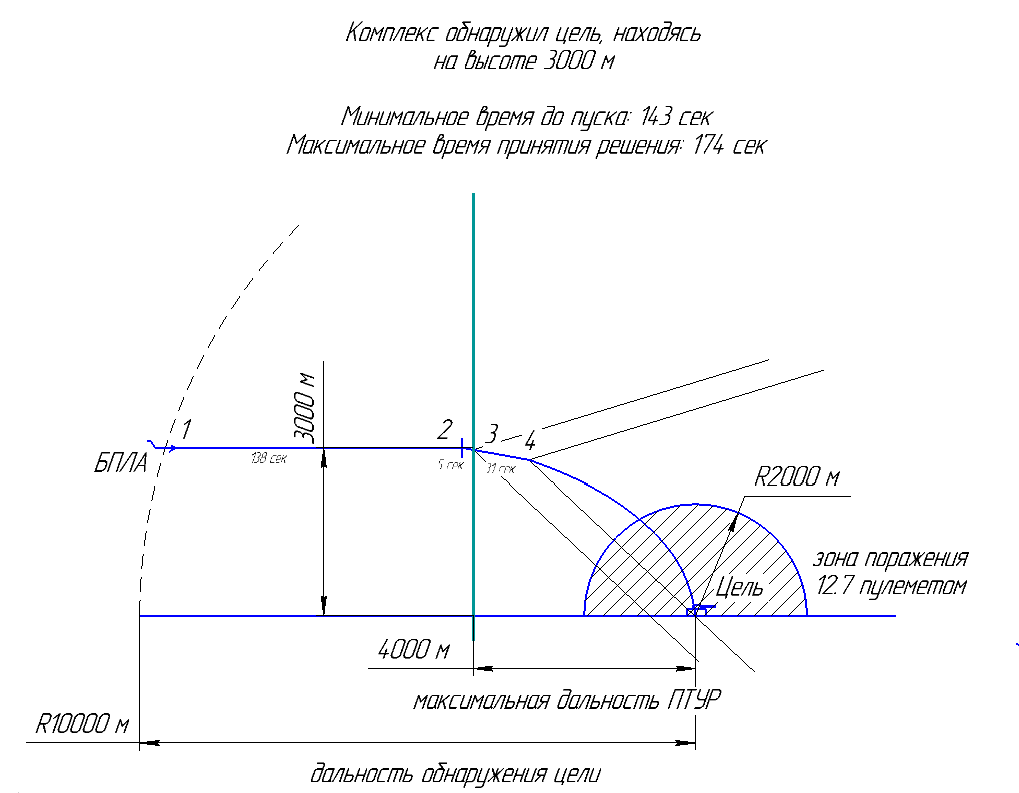
\includegraphics[width=\linewidth]{complex_works}
	\caption{Схема работы комплекса}
	\label{fig:complex_work_scheme}
\end{figure}


1 – цель попала в зону обнаружения БПЛА. Комплекс начинает движение в сторону цели;

2 – БПЛА выходит на пикирующий курс, позволяющий ПТУР быть направленной на цель после отделения;

3 – цель находится в зоне действия ПТУР, оператор БПЛА может принимать решение о запуске;

4 – цель находится в предельном положении, позволяющем ГСН ПТУР захватить цель после пуска. После выхода из этого положения пуск совершать не следует.

\clearpage
\subsection{Описание метода наведения ПТУР}
Для поражения цели сверху нужно применять особый метод наведения, так как «обычные» методы, например метод чистой погони, не позволят получить траекторию нужной формы.

В данном комплексе применяется метод погони с упреждением. Головка самонаведения обеспечивает угол обзора в 60 градусов. При отделении угол пеленга, обозначаемый $\alpha$, устанавливается максимальным значением вне зависимости от дальности. В зависимости от расстояния от точки пуска до цели, системой управления БПЛА просчитывается $t_{\text{нач}}$ и $t_{\text{кон}}$, которыми задается длительность манёвра и время его начала.
\begin{figure}[!h]
	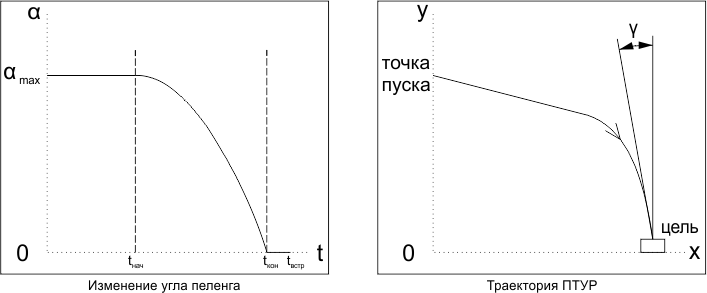
\includegraphics[width=\linewidth]{pre_hit_target}
	\caption{Изменение угла пеленга и траектория ПТУР}
	\label{fig:pre_hit_target}
\end{figure}

За счёт этого удается получить достаточно крутую траекторию и поразить цель в верхнюю проекцию. Важным критерием успешного поражения в данном случае является угол встречи с целью к вертикали, обозначаемый $\gamma$. Вид закона изменения угла пеленга и траектории представлен на рисунке \ref{fig:pre_hit_target}.

Определение оптимальных с точки зрения перегрузок, действующих на ПТУР, момента начала уменьшения угла пеленга уменьшения и скорости уменьшения – задача оптимизации, так как при слишком резком уменьшении пеленга ракета будет испытывать большие поперечные перегрузки, а при слишком слабом траектория будет слишком пологой и угол $\gamma$ может помешать её поражению. Подробная постановка и решение этой задачи подробно описаны в пункте \ref{cha:ch_2} (страница \pageref{cha:ch_2}).

В случае движения цели, целесообразно производить наведение в упрежденную точку, а в конце манёвра переводить наводить лазер на цель.
Наличие ГСН позволяет бороться с влиянием на поражение цели случайных возмущений, например ветра.

\clearpage
\section{Баллистическое проектирование ПТУР}
При решении задачи внешней баллистики определяются основные характеристики образца, которые должны соответствовать требованиям технического задания. В качестве основного критерия принимается минимум стартовой массы, при которой образец реализует доставку полезной нагрузки на необходимую дальность. При уменьшении веса ПТУР уменьшаются и ее габариты, что позволяет уменьшить расход материалов и затраты на изготовление конструкции образца.
\subsection{Исходные данные}
Исходные данные назначены в соответствии с классом разрабатываемого образца – ПТУР «воздух - поверхность» с силовой установкой РДТТ. Данные приведены в таблице \ref{tab:bal_proekt_nu}.

\begin{table}[!h]
	\begin{center}
		\caption{Исходные данные для баллистического проектирования}
		\begin{tabular}{|l|l|}
  		\hline
Дальность полета, км & 4000 \\ \hline
Высота пуска, км & 500 .. 4000 \\ \hline
Скорость пуска, км/ч & 150 км/ч \\ \hline
Число Маха на маршевом участке, M & 0,88 \\ \hline
		\end{tabular}
		\label{tab:bal_proekt_nu}
	\end{center}
\end{table}

В ходе баллистического проектирования ставится задача выбора оптимальной траектории ПТУР для полета на максимальную дальность. Для этого проварьируем высоты маршевого участка от 500 до 4000 м с шагом в 500 м. Лучший вариант будем определять по значению массы АУР, полученной при баллистическом проектировании.

Для образца на этапе баллистического проектирования совместно с решением задачи внешней баллистики проводится расчет параметров РДТТ, для чего необходимо располагать всей информацией о нем.

\subsection{Назначение параметров}
Калибр ПТУР назначаем из соотношения бронепробития и калибра, характерного для современных ПТУР:
\[ B = 6..8 \cdot d \]

Таким образом, $d = 800/6.8 = 117,7 \text{ мм}$. Принимаем диаметр кумулятивной воронки $d = 120 \text{ мм}$. Подробно расчет параметров БЧ описан в Приложении А на странице \pageref{cha:appendix_bch}. Зная калибр ПТУР, 
\begin{itemize}
	\item масса боевой части $m_{\text{бч}} = 2,2 \text{ кг}$;
	\item масса системы управления $m_{\text{су}} = 4,5 \text{ кг}$;
	\item масса полезной нагрузки $m_{\text{пн}} = m_{\text{бч}} + m_{\text{су}} = 6,7 \text{ кг}$;
	\item конструктивно-весовая характеристика $\beta = 1,4$;
	\item средняя скорость полета $V_{\text{ср}} = 290 \text{ м/с}$;
	\item тяговооруженность на стартовом участке $\eta_0 = 6$;
	\item удельный импульс топлива:    $I_{10} = 2400 \text{ (Н*с)/кг}$.
\end{itemize}
Параметры атмосферы принимаем принять постоянными невозможно, так как широк диапазон применения ПТУР по высоте. Давление, плотность и скорость звука в зависимости от высоты принимаем по ГОСТ 4401-81 (стандартная атмосфера).

\subsection{Система уравнений для решения\\задачи внешней баллистики}
Описание используемой системы уравнений подробно дано в пункте 7.4.1.

Системы уравнений записаны с учетом следующих допущений:
\begin{enumerate}[1.]
	\item Движение образца происходит в одной плоскости (вертикальной).
	\item Работа органов управления считается идеальной.
	\item Кривизна Земли и переменность ускорения свободного падения не учитываются.
	\item Движение образца описывается движением его центром масс (образец рассматривается как тяжелая материальная точка).
\end{enumerate}
\clearpage
Начальные условия для интегрирования на первом участке траектории:
\begin{itemize}
	\item t = 0 сек; V = 150 м/с (скорость носителя);
	\item х = 0 м; y = 3000 м (высота пуска);
	\item $\mu$ = 0.
\end{itemize}
Начальные условия для остальных участков определяются в результате расчетов на предыдущих участках.

Для решения задачи на активном участке траектории используется система уравнений (\ref{system:active}).

\begin{equation}
	\label{system:active}
	\left\{
			\begin{aligned}
			\frac{dV}{dt} & = \frac{g \cdot \eta}{1 - \mu} - i \cdot C_{43} \left( \frac{V}{\alpha(Y)} \right) \cdot \frac{\rho(Y)V^2g}{2q_{m0}(1-\frac{g*\eta}{J_{10}})} - g\sin \left[ \arctg \left( \frac{Y-Y_{\text{ц}}}{X-X_\text{ц}} \right) \right] ; \\
			\frac{dX}{dt} & = V \cdot \cos \left[ \arctg \left( \frac{Y-Y_{\text{ц}}}{X-X_\text{ц}} \right) \right] ; \\
			\frac{dY}{dt} & = V \cdot \sin \left[ \arctg \left( \frac{Y-Y_{\text{ц}}}{X-X_\text{ц}} \right) \right] .\\
			\frac{dm}{dt} & = \frac{g \cdot \eta}{J_{10}}
			\end{aligned}
	\right.
\end{equation}
Здесь $\alpha(t)$ - закон изменения угла пеленга; X, Y - текущие координаты ПТУР; $X_\text{ц}$, $Y_\text{ц}$ - координаты цели; $V$ - скорость ПТУР; $\eta$ - тяговооруженность; $\mu = \frac{dm}{dt}$ - расход топлива; $J_{10}$ - единичный импульс топлива; $a(Y)$ - скорость звука в зависимости от высоты полета; $C_{43}$ - функция 1943 года для определения лобового сопротивления ЛА.


Для решения задачи на пассивном участке траектории используется система уравнений (\ref{system:passive}).
\begin{equation}
	\label{system:passive}
	\left\{
			\begin{aligned}
			\frac{dV}{dt} & =  - i \cdot C_{43} \left( \frac{V}{\alpha(Y)} \right) \cdot \frac{\rho(Y)V^2g}{2q_{m0}} - g\sin \left[ \arctg \left( \frac{Y-Y_{\text{ц}}}{X-X_\text{ц}} \right) \right] ; \\
			\frac{dX}{dt} & = V \cdot \cos \left[ \arctg \left( \frac{Y-Y_{\text{ц}}}{X-X_\text{ц}} \right) \right] ; \\
			\frac{dY}{dt} & = V \cdot \sin \left[ \arctg \left( \frac{Y-Y_{\text{ц}}}{X-X_\text{ц}} \right) \right] .\\
			\frac{dm}{dt} & = 0
			\end{aligned}
	\right.
\end{equation}

На этапе баллистического проектирования величина $\alpha(t)$ (закон изменения угла пеленга) изменяется по закону, описанному в уравнении (\ref{system:rough_alpha}). На этапе баллистического проектирования проверяется соответствие диаграммы скорости требуемой форме и способность ПТУР поразить цель на максимальной дальности, поэтому закон $\alpha(t)$ выражен в виде кусочной линейной функции с произвольными участками.
\begin{equation}
	\label{system:rough_alpha}
	\alpha(t) = \begin{cases}
		25 & \text{, если t < 15} \\
		25 \cdot \dfrac{21 - t }{21-15} &  \text{, если } 15 \le t < 21 \\
		0 &  \text{, если t } \ge 21\\
	\end{cases}
\end{equation}

Изучение влияния $\alpha(t)$ на форму траектории и эффективность пражения цели более подробно описано в разделе \ref{chapter:traectory_optimization} на странице \pageref{chapter:traectory_optimization}.

\subsection{Результаты баллистического проектирования}
Результаты проектирования:
\begin{itemize}
	\item Стартовая масса ракеты:     m = 9,8 кг;
	\item Относительный запас топлива:    $\mu_0$ = 0,25;
	\item Запас топлива:       $\omega_0$ = 1,3 кг;
	\item Продолжительность стартового участка:  $t_0$ = 4.5 c;
	\item Секундный расход топлива:    $G_0$ = 0,31 кг;
	\item Средняя скорость полета:     $V_{\text{ср}}$ = 280,2 м/с;
	\item Начальная скорость:      $V_0$ = 42,0 м/с;
	\item Среднее время полета:     $t_\text{к}$ = 17,3 с;
	\item Потребная тяга:      $P_0$ = 680 Н;
	\item Полный импульс:      $I_P$ = 3300 Н $\cdot$ с.
\end{itemize}

Для старта с высоты 3100 м и расстояния до цели 4000 м приведена траектория полета движения (рисунок \ref{fig:sample_traectory}), a также графики изменения скорости ПТУР (рисунок \ref{fig:sample_speed}) и изменения угла пеленга (рисунок \ref{fig:sample_peleng}).
\clearpage

\begin{figure}[!h]
\begin{center}
	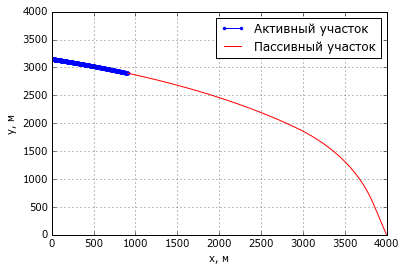
\includegraphics[height=8cm]{sample_traectory}
	\caption{Одна из возможных траекторий движения ПТУР}
	\label{fig:sample_traectory}
\end{center}
\end{figure}

\begin{figure}[h]
\begin{center}

	\begin{minipage}[h]{0.47\linewidth}
		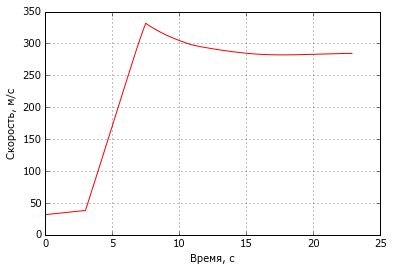
\includegraphics[width=1\linewidth]{sample_speed}
		\caption{Один из возможных графиков $V(t)$}
		\label{fig:sample_speed}
	\end{minipage}
	\hfill
	\begin{minipage}[h]{0.47\linewidth}
		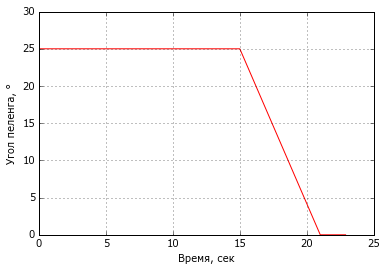
\includegraphics[width=1\linewidth]{sample_peleng}
		\caption{Принятая зависимость $\alpha(t)$}
		\label{fig:sample_peleng}
	\end{minipage}
\end{center}
\end{figure}

Графики отражают соответствие баллистического проектирования исходной задаче баллистического проектирования.

\clearpage
\section{Проектирование РДТТ}
На данном этапе проектирования ставится задача выбора конструктивных параметров двигательной установки стартовой ступени. В качестве топлива было выбрано нитраминное смесевое ТРТ (состав №13). Корпус ДУ выполнен из материала СП-33.

\subsection{Исходные данные}
Исходные данные основаны на результатах баллистического проектирования. В результате, были назначены следующие исходные данные:
\begin{itemize}
	\item Наружный диаметр корпуса ДУ:				$D_\text{н}$ = 125 мм;
	\item Полный импульс тяги стартового двигателя: $I_\text{п}$ = 3300 Н $\cdot$ c;
	\item Время работы двигателя:					$t_0$ = 4,5 с;
	\item Масса топлива двигателя:					$\omega_0$ = 1,3 кг;
\end{itemize}

\emph{Характеристики топлива (нитраминное смесевое ТРТ):}

\begin{itemize}
	\item Массовые доли и плотности компонентов топлива:
	\begin{enumerate}[1.]
		\item НТРВ:  		$g_1$ = 0,12; 		$\delta_1$ = 920  $\text{кг/м}^3$;
		\item ПХА:			$g_2$ = 0,62;		$\delta_2$ = 1950 $\text{кг/м}^3$;
		\item НМХ:			$g_3$ = 0,08;		$\delta_3$ = 1900 $\text{кг/м}^3$;
		\item Al:			$g_4$ = 0,18;		$\delta_4$ = 2700 $\text{кг/м}^3$;
	\end{enumerate}
	\item Плотность топлива:			$\delta=1/\sum_{i=1}^n \frac{g_i}{\delta_i} $=1794.8  $\text{кг/м}^3$;
	\item Тепловой эффект реакции:				Q = 5831,1 кДж/кг;
	\item Единичный импульс топлива:				$J_{40/1}$ = 2605,74 м/с;
	\item Температура продуктов сгорания:			$T_0$ = 3448,9 К;
	\item Показатель адиабаты:					k = 1,1821;
	\item Газовая постоянная газовой фазы:			$R_\text{г}$ = 428,77 Дж/кг $\cdot$ К;
	\item Массовая доля к-фазы в продуктах сгорания:	Z = 0,31947;
	\item Газовая постоянная смеси:		$R = R_\text{г}\cdot(1−Z)$ = 291,791 Дж/кг $\cdot$ К;
	\item Закон скорости горения:	$\xi=Z/(1-Z)=0,469$;
	\item Скорость горения при $p_{ref}$ = 5МПа:	$	u_{ref}$=6.0  мм/с;
	\item Показатель в степени закона горения:		$\nu$=0.25;
	\item Единичная скорость горения: $u_1=u_{ref} / p_{ref}^\nu$ = 4.012  мм/с;
	\item Термохимическая константа:				$D_t$=0.0025  1/(°C);
\end{itemize}

\emph{Характеристики материала корпуса ДУ (СП-33):}

\begin{itemize}
	\item Плотность материала					$\rho_\text{м}=7830  \text{кг/м}^3$ ;
	\item Временное сопротивление				$\sigma_\text{вр}=1650$ МПа ;
	\item Условный предел текучести			$\sigma_{0,2}=1350$ МПа ;
	\item Минимальная технологическая толщина стенки	$\delta_{min}$=1,5 мм;
\end{itemize}


\emph{Характеристики ТЗП:}

\begin{itemize}
	\item Плотность $\rho_\text{u}=1500  \text{кг/м}^3$ ;
	\item Толщина $\delta_u$=2,5 мм;
\end{itemize}

Расчет параметров ДУ приведен в Приложении Б (страница \ref{chapter:appendix_rdtt}).

При выборе наилучшего варианта ДУ в качестве основного критерия использовалась общая масса ДУ. В процессе сужения области поиска наилучшего решения во внимание принимались значения удельного импульса $I_{\text{уд}}$ и массы твердого топлива

\subsection{Результаты проектирования РДТТ}
Ниже представлены параметры выбранного варианта ДУ:
\begin{itemize}
	\item Давление в камере сгорания:				p = 7,6 МПа;
	\item Масса твердого топлива:					$\omega$ = 1.36 кг; 
	\item Удельный импульс:						$I_{10}$ = 2482 м/с; 
	\item Диаметр критического сечения сопла:			$d_{\text{кр}}$ = 10  мм; 
	\item Диаметр выходного сечения сопла:				$d_{\text{вых}}$ = 84 мм;
	\item Масса конструкции ДУ:					$m_{\text{кду}}$ = 2,5 кг; 
	\item К-т конструктивно-весового совершенства ДУ:		$\alpha$ = 0,289; 
	\item Толщина стенки корпуса ДУ:					$\delta$ = 1,5 мм; 
	\item Толщина слоя ТЗП:						$\delta u$ = 2,5 мм; 
	\item Минимальная толщина горящего свода заряда:		$e_1$ = 23 мм;
	\item К-т заполнения поперечного сечения заряда:		$\epsilon$ = 0,77.
\end{itemize}


\clearpage
\section{Аэродинамическое проектирование}
\subsection{Выбор аэродинамической схемы}
Основа выбора – анализ существующих схем: нормальной, утки, бесхвостки и поворотного крыла.

Для планеров, которым необходимо маневрировать на низких высотах рациональна компоновка в схеме «утка», в связи с тем, что данная схема обеспечивает лучшую манёвренность и управляемость.

\subsection{Центровочный расчет}
Центровкой называется процесс размещения грузов по корпусу изделия. При этом определяются центр тяжести, разбежка центра тяжести и моменты инерции изделия. В результате расчетов двигательной установки и предварительного проектирования образца была получена длина корпуса ракеты, равная L = 940 мм.

В таблице \ref{tab:center} приведены массы, длины и координаты центров тяжести отсеков ракеты. Координаты центра тяжести отсчитываются от носка корпуса. Также в таблице приведены весовые характеристики топлив каждой из двигательных установок.

\begin{table}[!h]
	\begin{center}
		\caption{Расрпеделение массы ПТУР по отсекам}
		\begin{tabular}{|l|p{25mm}|p{3cm}|p{35mm}|p{35mm}|}
  		\hline
№ &	Название отсека	& Масса отсека, m, кг & Длина отсека, l, мм & Центр тяжести отсека, X, мм \\ \hline
1 &	ГСН	& 0,8	& 172	& 130 \\ \hline
2 &	БЧ	& 3,1	& 205	& 305 \\ \hline
3 &	СУ и РМ	& 2,9	& 216 &	505 \\ \hline
4 &	РДТТ	& 2,5	& 288 &	690 \\  \hline
5 &	Сопловой блок	& 0,7	& 110 & 	820 \\ \hline
6 &	Топливо РДТТ	& 1,4 &	110	& 379 \\ \hline
		\end{tabular}
		\label{tab:center}
	\end{center}
\end{table}

\clearpage
\emph{Результаты центровочного расчета:}
\begin{itemize}
	\item Стартовая масса образца:					$m_0$ = 9,8 кг;
	\item Масса ракеты в конце активного участка:	$m_1$ = 8,4 кг;
	\item Центр тяжести ракеты на старте:			$X_{\text{цт полн}}$ = 488 мм;
	\item Центр тяжести «пустой» ракеты:			$X_{\text{цт пуст}}$ = 432 мм;
	\item Разбежка центра тяжести:					$\Delta X_\text{цт}$ = 57 мм;
	\item Относительная разбежка центра тяжести (\%):	$\Delta X_\text{цт}$ = 6,33\%;
	\item Момент инерции планера на старте:			$J_\text{z полн}$ = 931 Н$\cdot \text{м}^2$;
	\item Момент инерции «пустого» планера:			$J_\text{z пуст}$ = 604 Н$\cdot \text{м}^2$.
\end{itemize}

\subsection{Выбор геометрии планера}
В результате проектирования были получены следующие геометрические параметры планера:
\begin{itemize}
	\item Длина фюзеляжа:						$l_\text{ф} $ = 940 мм;
	\item Диаметр фюзеляжа:						d = 125 мм;
	\item Площадь миделева сечения:				$S_\text{м} $ = 0,012 м2;
	\item Длина головной части корпуса:			$l_\text{гч} $ = 172 мм;
	\item Длина кормовой части корпуса:			$l_\text{кч} $ = 768 мм;
	\item Удлинение фюзеляжа:					$\lambda_\text{ф} $ = 7,2;
	\item Удлинение головной части фюзеляжа:	$\lambda_\text{гч} $ = 1,37;
	\item Удлинение кормовой части фюзеляжа:	$\lambda_\text{кч} $ = 5,86;
	\item Сужение кормовой части фюзеляжа:		h = 0.
\end{itemize}

Определим площадь крыла исходя из величины потребной перегрузки и максимального угла атаки. Предельная перегрузка необходимая для маневра горка у подобного класса ракет обычно не превышает значения 6g. Поэтому примем:
\begin{itemize}
	\item Потребная перегрузка:					            $h_\text{потр}$ = 6;
	\item Максимальный угол атаки ЛА:			                $\alpha = 6\textdegree$;
	\item Средняя скорость полета:				            $V_\text{ср}$ = 280 м/с;
	\item Плотность воздуха на средней высоте полета (6 км):  $\rho_\text{в}$ = 0,75 $\text{кг/м}^3$;
	\item Коэффициент подъемной силы ЛА:	                  	$C_{y\alpha} $= 0,04.
\end{itemize}

Самое активное маневрирование ракета производит на маршевом и конечном участках полета, поэтому расчет будем производить для $m_1$. Таким образом, получаем:

\[
S_\text{кр}=\frac{n_\text{потр}m_1g}{C_y^\alpha \cdot \alpha \cdot \frac{\rho \cdot V^2}{2}}=0.19 \text{ м}^2.
\]

Для расчетов геометрии крыла примем следующие величины:
\begin{itemize}
	\item Относительное удлинение крыла:		$	\lambda_\text{кр} $ = 0,8;
	\item Относительное сужение крыла:			$	\eta_\text{кр} $= 3;
	\item Относительная толщина крыла:			$	\overline{c} $ = 5\%;
	\item Стреловидность передней кромки:		$	\chi_\text{пк}$ = 70°.
\end{itemize}

В результате расчетов была получены геометрические параметры крыла:
\begin{itemize}
	\item Размах крыла:							$l_\text{кр}$ = 0,195 м;
	\item Размах консолей крыла:					$l_\text{ккр}$ = 0,070 м;
	\item Площадь консолей крыла:					$S_\text{ккр}$ = 0,11 $\text{м}^2$;
	\item Относительное сужение консолей крыла:	$	\eta_\text{ккр}$ = 1,72;
	\item Относительное удлинение консолей крыла:	$	\lambda_\text{ккр}$ = 0,45;
	\item Средняя стреловидность:					$\chi_{0,5}$ = 57°;
	\item Средняя аэродинамическая хорда (САХ):	$	b_\text{a}$ = 0.315 м;
	\item Расстояние от САХ до оси ракеты:			$	z_\text{a}$ = 0,28 м;
	\item Бортовая хорда крыла:					$	b_\text{b}$ = 0,324 м;
	\item Корневая хорда крыла:					$	b_\text{0}$ = 0,460 м;
	\item Концевая хорда крыла:					$	b_\text{к}$ = 0,208 м;
	\item Стреловидность задней кромки:			$	\chi_\text{зк}$ = 0°.
\end{itemize}

\subsection{Расчет продольной устойчивости и управляемости}
Для расчета продольной устойчивости и управляемости необходимо определить аэродинамические силовые и моментные характеристики ЛА. Все расчеты проводились по методике изложенной в. Далее будут приведены расчеты для скорости 0,8 М, соответствующей полету у цели.

\paragraph{Коэффициент подъемной силы крыла, установленного на корпусе}

Входные параметры в графики:
\begin{enumerate}
	\item $\lambda_\text{ккр} \tg (\chi_{0,5}) = 0,675$;
	\item $\beta \lambda =\lambda_\text{ккр} \sqrt{(1-M^2 )} =0,62$;
	\item $\eta = \eta_\text{ккр}=1,785$.
\end{enumerate}

По графикам (1-6) [???] определяем: $K = \frac{C_y^\alpha \cdot 57.3}{\lambda} = 2,42$.
$$C_\text{y ккр}^\alpha = K \frac{\lambda_\text{ккр}}{57,3} = 0,019 $$

Крыло установлено не в конце корпуса, поэтому учитываем интерференцию:
$$ K_{\alpha\alpha} = \left[ 1 + \frac{d}{l_\text{кр}} \left(1,2 - \frac{0,2}{\eta_\text{ккр}}\right) \right]^2 = 1,997$$
Тогда $$C_\text{y кр}^\alpha = C_\text{y ккр}^\alpha K_{\alpha\alpha} \frac{S_\text{ккр}}{S_\text{кр}} = 0.016 \text{ } \frac{1}{\text{град}} $$

\paragraph{Фокус крыла, установленного на корпусе}
Входные параметры в графики:
\begin{enumerate}
	\item $\lambda_\text{ккр} \tg (\chi_{0,5}) = 0,675$;
	\item $\beta \lambda =\lambda_\text{ккр} \sqrt{(1-M^2 )} =0,62$;
	\item $\eta = \eta_\text{ккр}=1,785$;
	\item $\xi = \frac{d}{l_\text{кр}} = 0,373$.
\end{enumerate}

По графикам (7-11) [???] определяем: $\overline{\overline{X_\text{Fккр}}} =0,4$

По графику (12) [???] определяем: $K_1=0,7$
$$\Delta x = b_\text{бкр} - b_\text{акр} = -0,39 \text{ м.}$$

Тогда
$$
\overline{X_\text{Fккр}} = \frac{b_\text{бкр}}{b_\text{акр}} \left[ K_1 \overline{\overline{X_\text{Fккр}}} + 0,5(1-K_1) \left( 1 + \frac{d}{b_\text{бкр}} \sqrt{1 - M_0^2}  \right) \right] - 
\frac{\Delta x}{b_\text{акр}} = 0,69
$$

\clearpage
\paragraph{Коэффициент подъемной силы корпуса}

Входные параметры в графики:
\begin{enumerate}
	\item $ \dfrac{\lambda_\text{ккр}}{\lambda_\text{гч}} = 4,16$;
	\item $ \dfrac{\sqrt{1-M^2}}{\lambda_\text{гч}} = 0,481$;
\end{enumerate}

По графику (13) [???] определяем $C_\text{y гч}^\alpha = 0,052 \frac{1}{\text{град}} $ - коэффициент подъемной силы головной части;

$\alpha$ =0,15– коэффициент согласования

$d_\text{кч}=d=0,125$ м –диаметр кормовой части.

$C_\text{y кч}^\alpha=-0,035 \left(1-\dfrac{d_\text{кч}^2}{d^2} \right) a=0$ – коэффициент подъемной силы кормовой части.

$C_\text{y к}^\alpha=C_\text{y гч}^\alpha + C_\text{y кч}^\alpha = 0,052 \frac{1}{град}$ – коэффициент подъемной силы корпуса ракеты.

\paragraph{Центр давления корпуса}

Центр давления кормовой части: $X_\text{дкч}=l_\text{ф}- 0,5 l_\text{кч}=3,08$ м

Входные параметры в графики:
\begin{enumerate}
	\item $\dfrac{\lambda_\text{кч}} {\lambda_\text{гч}} =4,16$
	\item $\dfrac{\sqrt{1-М^2}}{\lambda_\text{гч}} =0,481$
\end{enumerate}

По графику (14) [???] определяем: $\Delta X_\text{1д}=0,2$

$\Delta X_\text{д}= \Delta X_\text{1д} l_\text{гч}=0.052 м$ – поправка на учет влияния цилиндрической части и сжимаемости.

$W_\text{гч}=\dfrac{1}{3} l_\text{гч} S_\text{м}=0,012 \text{ м}^3$ – объем головной части.

$X_\text{д кч}=l_\text{гч}- \frac{W_\text{гч}}{S_\text{м}} + \Delta X_\text{д}=0,086$ м – центр давления головной части.

$X_\text{дк}= \dfrac{X_\text{д кч} C_\text{y гч}^\alpha +C_\text{y кч}^\alpha X_\text{д кч} }{C_\text{y гч}^\alpha + C_\text{y кч}^\alpha } = 0,088$ м – положение центра давления корпуса относительно носка корпуса ракеты.

\clearpage
\paragraph{Коэффициент подъемной силы комбинации \\ крыла и корпуса}

Ранее были рассчитаны: 

$$C_\text{y к}^\alpha=0,052  \frac{1}{ \text{град} }, \text{  }  C_\text{y кр}^\alpha=0,016 \frac{1}{\text{град}} $$

Тогда

$$C_\text{y кр и к}^\alpha = C_\text{y к}^\alpha  \frac{S_\text{м}}{S_\text{кр}} + C_\text{y кр}^\alpha=0,021 \frac{1}{\text{град}}$$

\paragraph{Определение фокуса комбинации крыла и корпуса}

$X_\text{дк}=-1,95$ м– положение центра давления корпуса относительно носка САХ

$\overline{X_\text{дк}}= \frac{X_\text{дк}} {b_\text{акр}} =-1,4$ – относительная координата положения центра давления корпуса относительно носка САХ.

Ранее были рассчитаны: $C_\text{y к}^\alpha=0,052  \dfrac{1}{\text{град}} $;

$C_\text{y кр}^\alpha =0,016 \dfrac{1}{\text{град}}$ ; $\overline{X_F\text{кр}}=0,69$;

Тогда	$$\overline{X_\text{Fкр и к}} = \dfrac{\overline{X_\text{Fкр}} \cdot C_\text{y кр}^\alpha +  C_\text{y к}^\alpha \overline{X_\text{дк}} } {C_\text{y кр}^\alpha + C_\text{y к}^\alpha S_\text{м} }=0,166 $$.

\paragraph{Расчет площади оперения рулей}

Зададимся минимальным запасом статической устойчивости в начале движения изделия: $m_\text{z 0}$=-0,07.

Задача подбора площади оперения решается последовательными сближениями.

$X_\text{т0}$=-0.15 м – положение центра тяжести в конце полета относительно носка САХ.

$\overline{X_\text{т0}} = \dfrac{X_\text{т0}}{b_\text{акр}} $ =-0,1 – относительная координата положения центра тяжести в конце полета относительно носка САХ.

$\overline{ X_\text{Fкр и к} }=0,166 $– относительная координата положения фокуса комбинации крыла и корпуса в начале движения относительно носка САХ.

$L_\text{оп}=2,0$м – расстояние от центра тяжести до центра давления оперения.

$\overline{L_\text{оп}} = \dfrac{L_\text{оп}}{b_\text{акр}} $=1,43 – относительное расстояние от центра тяжести до центра давления оперения.

$m_\text{z б го}^{C_y} = \overline{X_\text{т0}} - \overline{X_\text{Fкр и к} } $ = -0,273 – степень устойчивости изделия без горизонтального оперения.

$$m_\text{z оп}^{C_y}=m_\text{z 0} - m_\text{z б го} ^{C_y} =0,2$$

$K_\text{т}$ = 0.9 – коэффициент торможения потока за крылом (рисунок 15) [???].

$\epsilon_\alpha $=0.65 – коэффициент скоса потока на оперение (рисунок 16) [???].

$$\overline{S_\text{оп}} = \dfrac{ m_\text{z оп}^{C_y} } { \overline{L_\text{оп}} \cdot K_\text{т} \cdot ( 1-\epsilon_\alpha) } =0,45$$

$$S_\text{оп}= \overline{S_\text{оп}} \cdot S_\text{кр}  = 0,41 \text{ м}^2$$


Принимаем площадь оперения равной Sоп = 0,4 м2. Для расчетов геометрии оперения примем следующие величины:
\begin{itemize}
 \item Относительное удлинение оперения:			$\lambda_\text{оп}$ = 1,5;
 \item Относительное сужение оперения:				$\eta_\text{оп} $= 2,2;
 \item Относительная толщина оперения:				$\overline{с} $ = 3 \%;
 \item Стреловидность передней кромки оперения:		$\chi_\text{пк оп} $ = 70º.
\end{itemize}

В результате расчетов была получены геометрические параметры крыла:
\begin{itemize}
 \item Размах оперения:							$l_\text{оп} $ = 0,190 м;
 \item Размах консолей оперения:				$	l_\text{коп} $ = 0,032 м;
 \item Площадь консолей оперения:				$	S_\text{коп} $ = 0,023 $\text{м}^2$;
 \item Относительное сужение консолей оперения:	$	\eta_\text{коп} $= 1,48;
 \item Относительное удлинение консолей оперения:	$	\lambda_\text{коп} $ = 1,74;
 \item Средняя стреловидность:					$\chi_\text{0,5 }$ = 2º;
 \item Средняя аэродинамическая хорда (САХ):	$		b_a $ = 0,072 м;
 \item Расстояние от САХ до оси ракеты:			$	z_a $ = 0,016 м;
 \item Бортовая хорда оперения:					$b_b $ = 0,082 м;
 \item Корневая хорда оперения:					$b_0 $ = 0,106 м;
 \item Концевая хорда оперения:					$b_\text{к} $ = 0,060 м;
 \item Стреловидность задней кромки:			$\chi_\text{зк} $= -30º.
\end{itemize}

\paragraph{Коэффициент подъемной силы оперения}

Входные параметры в графики:
\begin{enumerate}
	\item $\lambda_\text{коп} \tg \left( \chi_{05} \right)$ = 2,607;
	\item $\beta\lambda = \lambda_\text{коп} \sqrt{1 - M^2} = $ 2,4;
	\item $\eta = \eta_\text{коп} = $ 1.5.
\end{enumerate}

По графикам (1-6) [???] определяем: $K = \frac{C_y^\alpha \cdot 57.3}{\lambda} = 1,4$.
$$C_\text{y коп}^\alpha = K \frac{\lambda_\text{коп}}{57,3} = 0,043 $$

Оперение установлено в конце корпуса, поэтому не учитываем интерференцию.
Тогда $C_\text{y оп}^\alpha = C_\text{у коп}^\alpha  \frac{S_\text{коп}}{S_\text{кр}}  =0.0027  \frac{1}{\text{град}} $

\paragraph{Фокус оперения, установленного на корпусе}

Входные параметры в графики:
\begin{enumerate}
	\item $\lambda_\text{коп} \tg (\chi_{0,5}) = 0,675$;
	\item $\beta \lambda =\lambda_\text{коп} \sqrt{(1-M^2 )} =0,62$;
	\item $\eta = \eta_\text{коп}=1,785$;
	\item $\xi = \frac{d}{l_\text{кр}} = 0,373$.
\end{enumerate}

По графикам (7-11) [???] определяем: $\overline{\overline{X_\text{Fкоп}}} =0,55$

По графику (12) [???] определяем: $K_1=0,75$
$$\Delta x = b_\text{боп} - b_\text{аоп} = -0,06 \text{ м.}$$

Тогда
$$
\overline{X_\text{Fоп}} = \frac{b_\text{боп}}{b_\text{аоп}} \left[ K_1 \overline{\overline{X_\text{Fоп}}} + 0,5(1-K_1) \left( 1 + \frac{d}{b_\text{боп}} \sqrt{1 - M_0^2}  \right) \right] - 
\frac{\Delta x}{b_\text{аоп}} = 0,271
$$

\paragraph{Уточнение величины запаса статической устойчивости}

$X_\text{Fоп} $=-0,61 – координата центра давления оперения от носка САХ.

$\overline{X_\text{Fоп} }=X_\text{Fоп}/b_\text{акр} $=-1,4 – относительная координата центра давленияоперения от носка САХ.

$\overline{ \Delta X_\text{Fоп} } = \dfrac {-\overline{X_\text{Fкр и к}}+\overline{X_\text{Fоп}} } { 1+ \dfrac{ C_\text{y кр и к}^\alpha} {C_\text{y оп}^\alpha } }$=0,015 – смещение фокуса комбинации крыла и корпуса оперением.

$\overline{X_{F0}}= \overline{X_\text{Fкр и к}} +\overline{\Delta X_\text{Fоп}} $=0,181 – относительная координата начального положения фокуса оперения от носка САХ.

$\overline{X_\text{т0} } $ = -0,107 – относительная координата начального положения центра тяжести от носка САХ.

Уточним значение запаса статической устойчивости:

$$m_{z0}^{Cy} = \overline{X_\text{т0}} - \overline{X_\text{F0}} = \text{ -0,09} $$

\paragraph{Коэффициент подъемной силы всего изделия}

Ранее были рассчитаны: $C_\text{y оп}^\alpha=0,0027$ $ \dfrac{1}{\text{град}}$;  $C_\text{y кр и к}^\alpha=0,021$ $\dfrac{1}{\text{град}}$

Коэффициент подъемной силы всего изделия при нулевом угле атаки:

$C_\text{y0}^\alpha = C_\text{y оп}^\alpha+C_\text{y кр и к}^\alpha $= 0,024  $\dfrac{1}{\text{град}}$.

Тогда коэффициент подъемной силы ЛА при угле атаки $\alpha$ = 5º равен:
$$C_y=C_\text{y0}^\alpha \cdot \alpha  = 0,119$$


\paragraph{Определение балансировочной зависимости и выбор рулей}

В нашем случае основным органом управления является оперение ($S_\text{р} = S_\text{коп} = 0,225 \text{ м}^2$).

Входные параметры в графики:
\begin{enumerate}
	\item $\eta=\eta_\text{коп} $=1,48;
	\item $\xi=\dfrac{d}{l_\text{оп}} $ =0,32.
\end{enumerate}

По графикам (17) [???]  определяем: $K_\delta$=1,5

По графику (18) [???]  определяем:$K_\eta$=0,75

$\phi=1+K_\eta(M-1)$=1,53;
$C_\text{y р}^\delta=C_\text{y оп}^\alpha \cdot \phi \cdot K_\delta $=0,049 $\dfrac{1}{\text{град}}$;

$\overline{S_\text{р} }=S_\text{коп}/S_\text{кр}$ = 0,2 – относительная площадь руля.

$\overline{L_\text{р} }=\overline{X_\text{т0}}-\overline{X_\text{Fоп}}$ =-1,46 – относительное расстояние от центра давления руля до центра тяжести изделия.

$m_{z_0}^{C_{y}} $ = -0,09 – запас статической устойчивости.

$ \delta(\alpha)= \dfrac{-C_y^\alpha \cdot m_{z0}^{Cy} } {C_\text{y р}^\delta \cdot \overline{S_\text{р}} \cdot \overline{L_\text{р}} \cdot К_\text{т} } \alpha $ – балансировочная зависимость.
$\alpha $=5° – угол атаки.

$ \frac{\delta(\alpha)}{\alpha} $= -0,9 – значение балансировочной зависимости при заданном угле атаки.

Кроме этого, были получены балансировочные зависимости в начале управляемого участка полета  $\frac{\delta(\alpha)}{\alpha}$= =-1,3. Полученые значения удоволетворяют рекомендованному диапазону для «нормальной схемы» $\left( \dfrac{\delta(\alpha)}{\alpha}=-0,6 \div -1,5 \right) $.

Проверим возможность применения ЛА при полученных балансировочных зависимостях.

$Q_1 $ = 992 Н– вес ракеты перед маршевым участком.

$n_\text{ур}$ = 6 – максимальная поперечная перегрузка на данном участке полета.

$q_1$ = 74500  $\frac{\text{кг}}{м \cdot c^2} $ – скоростной напор.

$Y_{\alpha.p}=1.1 C_{y1}^\alpha S_\text{кр} q_1 $ = 2000 Н – подъемная сила ЛА.

Необходимый угол поворота рулей:

$$\delta_\text{потр} = \dfrac{Q_1 n_\text{ур}}{Y_{\alpha.p}} = 23,5\text{°}$$

Потребный угол атаки: $\alpha_\text{потр} $ = 8°
$$\delta_\text{потр}-\alpha_\text{потр} = 15,5\text{°}$$

Разница между углом поворота руля и углом атаки меньше 20º, значит применение ЛА в данных условиях возможно

\clearpage
\subsection{Определение динамических характеристик планера}

$\tau= \dfrac {2 \cdot m_\text{пуст}} {\rho \cdot V \cdot S_\text{кр} }  = 0,935$ с – параметр времени.

$\overline{r_z} = \dfrac{1}{b_\text{акр}}  \sqrt{\dfrac{J_z} {m_\text{пуст}}}  = 0,92 $  м – безразмерный радиус инерции на старте.

$\mu= \dfrac{ 2 \cdot m_\text{пуст}} {\rho \cdot S_\text{кр} \cdot b_\text{акр} }  = 387$ – коэффициент относительной плотности.

Коэффициент демпфирования:

Ранее были расчитаны: $C_y^\alpha=0,024; m_z^{\omega z} = -0,96; m_z^\alpha = -0,155;$

$$h= \dfrac{1}{2} \cdot \dfrac{1}{\tau} \left[C_y^\alpha \cdot 57,3- \dfrac{m_z^{\omega z}+m_z^\alpha} {\overline{r_z}^2} \right]=1,43 \text{ }  \dfrac{1}{c} $$

Собственная угловая частота планера:

$$\Omega= \sqrt{ \frac{C_y^\alpha \cdot 57,3}{\tau^2} \cdot \frac{m_z^\omega z+\mu\cdot m_z^\alpha}{\overline{r_z}^2} } \text{ } \dfrac{1}{c}$$

Коэффициент относительного демпфирования: $\eta=\dfrac{h}{\Omega}=0,194 $.

В результате видно, что коэффициент относительного демпфирования у цели попадает в диапазон рекомендованных значений $0,1 < \eta < 0,8$. Кроме этого были рассчитаны коэффициенты относительного демпфирования для остальных участков полета, которые так же находятся в допустимых значениях.

\subsection{Определение шарнирных моментов органов управления}
$C_\text{y р}^\alpha=C_\text{y коп}^\alpha = 0,043$ – коэффициент подъемной силы руля.

$C_\text{y р}^\delta=0,049 $ – коэффициент подъемной силы руля, возникающий при его повороте.

$X_\text{ов}=1,8$ м –координата оси вращения руля от носка САХ.

$\overline{X_\text{ов}}= \frac{X_\text{ов}} {b_\text{акр}}  =-0,081$ – относительная координата оси вращения руля относка САХ.

$\overline{X_\text{доп} }=-0,099$  – относительная координата центра давления руля относка САХ.
$$m_\text{ш}^\delta=-C_\text{y р}^\delta (\overline{X_\text{доп}}-\overline{X_\text{ов}})=-0,0055 $$
$$m_\text{ш}^\alpha=-C_\text{y р}^\alpha (\overline{X_\text{доп}}-\overline{X_\text{ов}})=-0,0049 $$
коэффициенты шарнирного момента.
$$m_\text{ш.0} (\alpha,\delta)=m_\text{ш}^\delta \cdot \delta+m_\text{ш}^\alpha \cdot \alpha$$

$\alpha=5°$ – угол атаки.

$\delta(\alpha)=-4,5°$ – угол поворота руля.

$m_\text{ш} (\alpha,\delta(\alpha))=-0,028 $ – коэффициент шарнирного момента при заданном угле атаки.

$M_\text{ш} (\alpha,\delta)=m_\text{ш} (\alpha,\delta) \cdot q \cdot S_\text{ккр} \cdot b_\text{аккр} $ – шарнирный момент.

$M_\text{ш} (\alpha,\delta(\alpha))=-1,2$ Н $\cdot$ м – шарнирный момент, при заданном угле атаки.

При конструировании ракеты были выбраны индукционные привода для управления рулями. Данный тип приводов выдерживает рассчитывает шарнирный момент.

\subsection{Расчет лобового сопротивления ПТУР}

\paragraph{Коэффициент лобового сопротивления корпуса}

Выполним предварительные вычисления:

$F_\text{кч}=\pi d l_\text{кч}=4,574 \text{ м}^2$ – площадь кормовой части.

$F_\text{гч}=\frac{1}{2} \pi d l_\text{гч}=0,55 \text{ м}^2$ – площадь головной части

$F_\text{к}=F_\text{кч}+F_\text{гч}=5,124 \text{ м}^2$ – площадь смачиваемой поверхности корпуса.

$\eta_c = 1 + \frac{1}{\lambda_\text{гч}} =1,35$ – коэффициент, учитывающий влияние формы корпуса.
$C_\text{хкч}=0 $– коэффициент волнового сопротивления кормовой части.

$C_\text{хд}=0 $– коэффициент донного сопротивления корпуса.

Донное сопротивление отсутствует, так как по всей траектории полета двигатель находится в рабочем состоянии.

$Re_\text{к}=V \frac{l_\text{ф}}{\nu}=2,1 \cdot 10^9 $ – число Рейнольдса.

Тогда $C_{xf}=\frac{0,074}{Re^{0,2}} =10^{-3}$– коэффициент сопротивления трения для плоской пластины.

$\eta_\text{м} = \dfrac{1} {1+0,1615 (M-0,25)^{1,325}} =0,79$ – коэффициент учитывающий сжимаемость.

$C_{xfk} = C_{xfl} \dfrac{F_\text{к}} {S_\text{м}}  \eta_\text{м} \eta_c =0,057$ – коэффициент сопротивления трения.

$C_\text{хгч}=(0,0016+0,002M^{-2} )  \Theta_\text{к}^{1.7}=0.481$ – коэффициент волнового сопротивления головной части.

$C_\text{хвк}=C_\text{хгч}+C_\text{хкч}=0,373$ – коэффициент волнового сопротивления корпуса.

$C_\text{х.0.к}=C_{xfk}+C_\text{хвк}+C_\text{хд}=0,431 $– Коэффициент лобового сопротивления корпуса (при нулевом угле атаки).

\paragraph{Коэффициент лобового сопротивления крыла}

$\eta_\text{скр}=1$ – поправка на учет формы профиля.

$n = 2$ – число пар консолей крыла.

$Re_\text{кр}=V \dfrac{b_\text{акр}}{\nu}=5,8 \cdot 10^8 $ – число Рейнольдса

$C_{xfl}=\dfrac{0.455}{\ln \left(Re_\text{кр.0}\right)^2.58} = 2,0 \cdot 10^{-4} $– коэффициент сопротивления трения для плоской пластины.

$C_{xfkp}=C_{xfl} \dfrac{S_\text{ккр}} {S_\text{кр}}  \eta_\text{м} \eta_\text{скр}=6,7 \cdot 10^{-5} $ – коэффициент сопротивления трения.

Входные параметры в графики:
\begin{enumerate}
	\item $\lambda_\text{ккр} \tg \left( \chi_{0,5\text{кр}} \right) =0,675 $
	\item $\lambda_\text{ккр} \sqrt{1-M_0^2} =0,62$
	\item $\lambda_\text{ккр} \sqrt[3]{c_\text{кр.отн}} =0,14$
	\item $\eta_\text{ккр}=1,785$
\end{enumerate}

По графикам (25-27) [???] определяем: $C_\text{хв}/(\lambda c^2 )=1,8$

$$C_\text{хвкр}=0.87 \lambda_\text{ккр}  c_\text{кр.отн}^2 K =6,3 \cdot 10^{-4}$$

$\lambda_\text{ккр} \sqrt{1-M_0^2} - \lambda_\text{ккр} \tg \left( \chi_{0,5\text{кр}} \right) =-0,055 $   Поэтому  $\phi = 1$

Так как крыло ромбовидное, K=1

$C_\text{хвкр}=C_\text{хвкр} [1+\phi(K+1)] = 6,4 \cdot 10^{-4} $– коэффициент волнового сопротивления крыла.'

Так как надстроек на крыле нет, то  $\Delta C_\text{хкр}=0$

$ C_\text{х.0.кр}=C_{xfkp}+C_\text{хвкр}+ \Delta C_\text{хкр}=0,0007$ – Коэффициент лобового сопротивления крыла(при нулевом угле атаки).

\paragraph{Коэффициент лобового сопротивления оперения}

$\eta_\text{соп}=1$ – поправка на учет формы профиля.

$n=2$ – число пар консолей крыла.

$Re_\text{оп}=V \dfrac{b_\text{аоп}} {\nu} =1,7 \cdot 10^8$ – число Рейнольдса

$C_{xfl}= \dfrac{0.455} { \left( \ln \left(Re_\text{оп.0}\right) \right)^2.58} = 2,3 \cdot 10^{-4} $ – коэффициент сопротивления трения для плоской пластины.

$ C_\text{xfоп}=C_{xfl} \dfrac{S_\text{коп}}{S_\text{оп} } \eta_\text{м} \eta_\text{соп} = 1,02 \cdot 10^{-4}$ – коэффициент сопротивления трения.

Входные параметры в графики:
\begin{enumerate}
	\item $\lambda_\text{коп}  \tg \left( \chi_\text{0,5оп} \right) =2,6 $;
	\item $\lambda_\text{коп} \sqrt{1-M_0^2}=2,4$;
	\item $\lambda_\text{коп} \sqrt[3]{c_\text{оп.отн}} =0,54$;
	\item $\eta_\text{коп} = 1,48$.
\end{enumerate}

По графикам (25-27) [???]  определяем: $C_\text{хв}/(\lambda c^2 )=K=0,8$

$C_\text{хвоп}=0,87\lambda_\text{коп}  c_(оп.отн)^2 K=1,1 \cdot 10^{-3}$

$\lambda_\text{коп} \sqrt{1-M_0^2}-\lambda_\text{коп}  \tg \left(\chi _\text{0,5оп} \right)=-0,21 $. Поэтому  $\phi=1$.

Так как оперение ромбовидное, K=1

$C_\text{хвоп} = C_\text{хвоп} [1+ \phi (K+1)]=1,1 \cdot 10^{-3}  $– коэффициент волнового сопротивления крыла.

Так как надстроек на крыле нет, то  $\Delta C_\text{хоп}=0 $

$C_\text{х.0.оп}=C_\text{xfоп}+C_\text{хвоп}+ \Delta C_\text{хоп}=0,0012 $– Коэффициент лобового сопротивления крыла(при нулевом угле атаки).

\paragraph{Коэффициент лобового сопротивления изделия (при нулевом угле атаки)}

$$C_\text{х.0}=C_\text{х.0.к}+C_\text{х.0.кр} \frac{S_\text{кр}} {S_\text{м}} +C_\text{х.0.оп}  \frac{S_\text{оп}} {S_\text{м} } =0,45$$

Из полученных результатов видно, что коэффициент лобового сопротивления в целом согласовывается со значениями, которые использовались в баллистическом проектировании. 
